\documentclass[12pt,a4paper]{article}

% --- Persian/RTL Support (XePersian) ---
% hyperref must be loaded before xepersian/bidi
\usepackage{hyperref}
\usepackage{xepersian}
\settextfont{Vazirmatn}[Scale=1.1]
\setdigitfont{Vazirmatn}[Scale=1.1]
\setlatintextfont{Libertinus Serif}
\setmonofont{Vazirmatn}

% \foreignlanguage was provided by polyglossia; keep it working via \lr
\renewcommand{\foreignlanguage}[2]{\lr{#1}}

% --- Page Layout ---
\usepackage[a4paper, top=2.5cm, bottom=2.5cm, left=2.5cm, right=2.5cm, headheight=15pt]{geometry}
\usepackage{setspace}
\onehalfspacing
\usepackage{titlesec}
\usepackage{fancyhdr}
\usepackage{lastpage}
\usepackage{xcolor}
\hypersetup{
  colorlinks=true,
  linkcolor=blue,
  citecolor=blue,
  urlcolor=blue,
  pdftitle={امنیت و حفاظت در  شبکه اقتضایی خودرویی},
  pdfauthor={سید علی موسوی},
  bookmarks=true,
  bookmarksnumbered=true,
  bookmarksopen=true,
}

% --- Headers and Footers ---
\pagestyle{fancy}
\fancyhf{}
\fancyhead[L]{\small\leftmark}
\fancyhead[R]{\small حریم خصوصی و امنیت در  شبکه اقتضایی خودرویی}
\fancyfoot[C]{\small صفحه \thepage\ از \pageref{LastPage}}
\renewcommand{\headrulewidth}{0.4pt}
\renewcommand{\footrulewidth}{0.4pt}

% --- Section Formatting ---
\titleformat{\section}{\Large\bfseries}{\thesection}{1em}{}
\titleformat{\subsection}{\large\bfseries}{\thesubsection}{1em}{}
\titleformat{\subsubsection}{\normalsize\bfseries}{\thesubsubsection}{1em}{}

% --- Math Packages ---
\usepackage{amsmath}
\usepackage{amssymb}
\usepackage{tikz}

% --- Table and Figure Packages ---
\usepackage{booktabs}
\usepackage{tabularx}
\usepackage{graphicx}
\usepackage{float}
\usepackage{caption}
\captionsetup{font=small, labelfont=bf}

% --- Lists ---
\usepackage{enumitem}
\setlist[itemize]{noitemsep, topsep=0pt}

% --- Line Spacing ---
\usepackage{leading}
\leading{18pt}

% --- Graphics Path ---
\graphicspath{{images/}}

% --- Bibliography ---
\usepackage[
    backend=biber,
    style=ieee,
    sorting=none
]{biblatex}

\addbibresource{report.bib}

% English, left-aligned bibliography numbers
\DeclareFieldFormat{labelnumberwidth}{\makebox[2em][l]{\lr{[#1]}}}

% --- Footnotes ---
\makeatletter
\renewcommand{\footnoterule}{%
  \kern-3pt
  \hrule width \textwidth
  \kern 2.6pt
}
\makeatother

% Paragraph formatting
\setlength{\parindent}{0pt}
\setlength{\parskip}{6pt}

% --- Title Page Info ---
\title{
  \vspace{-1cm}
  {\Huge\bfseries حریم خصوصی و امنیت در شبکه اقتضایی خودرویی} \\
}

\author{
  \vspace{1cm}
  {\large دانشکده مهندسی کامپیوتر} \\
  \vspace{1cm}
  {\large دانشجو: سید علی موسوی} \\
  \vspace{0.5cm}
  {\large استاد راهنما: دکتر بابک صادقیان} \\
  \vspace{0.5cm}
  {\large استاد درس سمینار: دکتر رضا صفابخش}
}

\date{\vspace{1cm}مرداد ماه ۱۴۰۵}

\begin{document}

% --- Persian Title ---
\begin{titlepage}
\begin{center}
\vspace*{0.5cm}

% University Logo

\includegraphics[width=3cm]{images/amirkabir_logo-1.png}

\vspace{0.5cm}

{\Large\textbf{دانشگاه صنعتی امیرکبیر (پلی‌تکنیک تهران)}} \\[0.3cm]
{\large\textbf{دانشکده مهندسی کامپیوتر}} \\[1.5cm]

{\Huge\textbf{حریم خصوصی و امنیت در شبکه اقتضایی خودرویی}} \\[1.5cm]

{\large\textbf{گزارش سمینار کارشناسی ارشد}} \\[1cm]

\begin{tabular}{rl}
\textbf{دانشجو:} & سید علی موسوی \\[0.3cm]
\textbf{استاد راهنما:} & دکتر بابک صادقیان \\[0.3cm]
\textbf{استاد درس سمینار:} & دکتر رضا صفابخش \\
\end{tabular}

\vspace{1.5cm}
{\large مردادماه ۱۴۰۵}

\end{center}
\end{titlepage}

% --- Abstract ---
\newpage
\begin{abstract}
شبکه‌های اقتضایی خودرویی \LTRfootnote{\lr{Vehicular Ad-hoc Networks (VANET)}} به عنوان بخشی از سیستم‌های حمل‌ونقل هوشمند، با امکان تبادل اطلاعات بین خودروها و زیرساخت‌های جاده‌ای، نقش بسیار مهمی در بهبود ایمنی ترافیک و کاهش تصادفات ایفا می‌کنند. با این حال، ماهیت بی‌سیم و باز این شبکه‌ها، آن‌ها را در برابر حملات امنیتی مختلف مانند حملات جعل پیام، حملات سیبل، حملات مرد میانی و نقض حریم خصوصی آسیب‌پذیر می‌سازد. در این گزارش، ابتدا معماری و ویژگی‌های شبکه‌های اقتضایی خودرویی  مورد بررسی قرار می‌گیرد و سپس چالش‌های امنیتی موجود در این شبکه‌ها تحلیل می‌شود. فناوری بلاکچین به عنوان یک راهکار غیرمتمرکز برای حل مشکلات اعتماد و امنیت در شبکه‌های اقتضایی خودرویی  معرفی شده و محدودیت‌های آن در این حوزه بررسی می‌شود. \lr{IOTA Tangle} به عنوان جایگزینی مقیاس‌پذیر و بدون کارمزد برای بلاکچین‌های سنتی مورد بحث قرار می‌گیرد. در نهایت، مفاهیم مدیریت هویت، شبه‌نام، هویت خودمختار \LTRfootnote{\lr{Self-Sovereign Identity (SSI)}} و شناسه‌های غیرمتمرکز \LTRfootnote{\lr{Decentralized Identifiers (DID)}} به عنوان راهکارهای نوین برای حل مشکلات امنیتی و حفظ حریم خصوصی در شبکه‌های اقتضایی خودرویی ارائه می‌شوند. همچنین نقش روش‌های هوش مصنوعی در تقویت امنیت  شبکه اقتضایی خودرویی مورد توجه ویژه قرار گرفته است.
\end{abstract}

\newpage

\tableofcontents
\newpage

% ========================================================================
% فصل اول: مقدمه
% ========================================================================
\section{مقدمه}
شبکه اقتضایی خودرویی \LTRfootnote{\lr{Vehicular Ad-hoc Networks (VANET)}} یکی از مهمترین فناوری‌های حوزه سیستم‌های حمل‌ونقل هوشمند است. این شبکه‌ با امکان تبادل اطلاعات بین خودروها و زیرساخت‌های جاده‌ای، نقش بسیار مهمی در بهبود ایمنی ترافیک، کاهش تصادفات و افزایش بهره‌وری حمل‌ونقل ایفا می‌کنند \cite{hozouriOverviewVANETVehicular2023}.

بر اساس آمار سازمان بهداشت جهانی، سالانه بیش از ۱.۱۹ میلیون نفر در تصادفات جاده‌ای جان خود را از دست می‌دهند و تصادفات جاده‌ای مهمترین عامل مرگ کودکان و جوانان ۵ تا ۲۹ ساله است \cite{farsimadanReviewSecurityChallenges2025}. بیش از ۹۲ درصد تصادفات به خطای انسانی نسبت داده می‌شود \cite{hozouriOverviewVANETVehicular2023}. در این راستا،  شبکه اقتضایی خودرویی با امکان ارائه هشدارهای ایمنی بلادرنگ و اطلاعات ترافیکی، پتانسیل بالایی برای کاهش این آمار دارند.

با این حال، ماهیت بی‌سیم و باز ارتباطات در  شبکه اقتضایی خودرویی، این شبکه‌ها را در برابر تهدیدات امنیتی مختلف آسیب‌پذیر می‌سازد. حملات جعل پیام، حملات سیبل، حملات مرد میانی و نقض حریم خصوصی از جمله مهمترین چالش‌های امنیتی در این حوزه هستند \cite{farsimadanReviewSecurityChallenges2025, VanetSecurityPrivacy}.

در سال‌های اخیر، فناوری بلاکچین به عنوان یک راهکار غیرمتمرکز برای حل مشکلات اعتماد و امنیت در  شبکه اقتضایی خودرویی مورد توجه قرار گرفته است \cite{razaBlockchainBasedReputationTrust2024, fengBPASBlockchainAssistedPrivacyPreserving2020}. با این حال، بلاکچین‌های سنتی نیز محدودیت‌هایی مانند مقیاس‌پذیری پایین و مصرف انرژی بالا دارند که \lr{IOTA Tangle} به عنوان جایگزینی مناسب برای رفع این مشکلات معرفی شده است \cite{IOTATANGLE20, silvanoIotaTangleCryptocurrency2020}.

همچنین، مدیریت هویت و حفظ حریم خصوصی از مهمترین دغدغه‌های کاربران  شبکه اقتضایی خودرویی است. فناوری‌های نوین مانند هویت خودمختار \LTRfootnote{\lr{Self-Sovereign Identity (SSI)}}، شناسه‌های غیرمتمرکز \LTRfootnote{\lr{Decentralized Identifiers (DID)}} و اعتبارنامه‌های تأییدپذیر \LTRfootnote{\lr{Verifiable Credentials (VC)}} به عنوان راهکارهایی برای حل مشکلات مدیریت هویت و شبه‌نام در  شبکه اقتضایی خودرویی مطرح شده‌اند \cite{mazzocca2025survey, feraudoDIVADIDbasedReputation2024}.

این گزارش با هدف مرور جامع بر چالش‌های امنیتی در شبکه اقتضایی خودرویی و ارائه راهکارهای موجود تهیه شده است. در ادامه، ابتدا مفهوم  شبکه اقتضایی خودرویی و اهمیت آن بیان می‌شود، سپس محدودیت‌ها و چالش‌های موجود بررسی می‌گردد و در نهایت راهکارهای مبتنی بر بلاکچین، \lr{IOTA Tangle} و مدیریت هویت مورد بحث قرار می‌گیرند.

% ========================================================================
% فصل دوم: VANET چیست؟
% ========================================================================
\section{شبکه اقتضایی خودرویی چیست؟}

\subsection{تعریف و مفهوم}

شبکه اقتضایی خودرویی یک زیرمجموعه از شبکه‌های خودمختار متحرک \LTRfootnote{\lr{Mobile Ad-hoc Networks (MANET)}} است که ارتباط بین خودروهای نزدیک و بین خودروها و زیرساخت‌ها را تسهیل می‌کند \cite{hozouriOverviewVANETVehicular2023}. در این شبکه‌ها، خودروها به عنوان گره‌های متحرک عمل کرده و اطلاعات ایمنی و ترافیکی را با یکدیگر به اشتراک می‌گذارند \cite{xuInternetVehiclesBig2018}. خودروهای متصل با امکان ارتباط با محیط داخلی و خارجی خود، بخشی جدایی‌ناپذیر از زندگی مدرن شده‌اند و پیش‌بینی می‌شود بازار جهانی خودروهای متصل تا سال ۲۰۱۹ به ۱۳۱.۹ میلیارد دلار برسد \cite{luConnectedVehiclesSolutions2014}.

\begin{figure}[H]
\centering
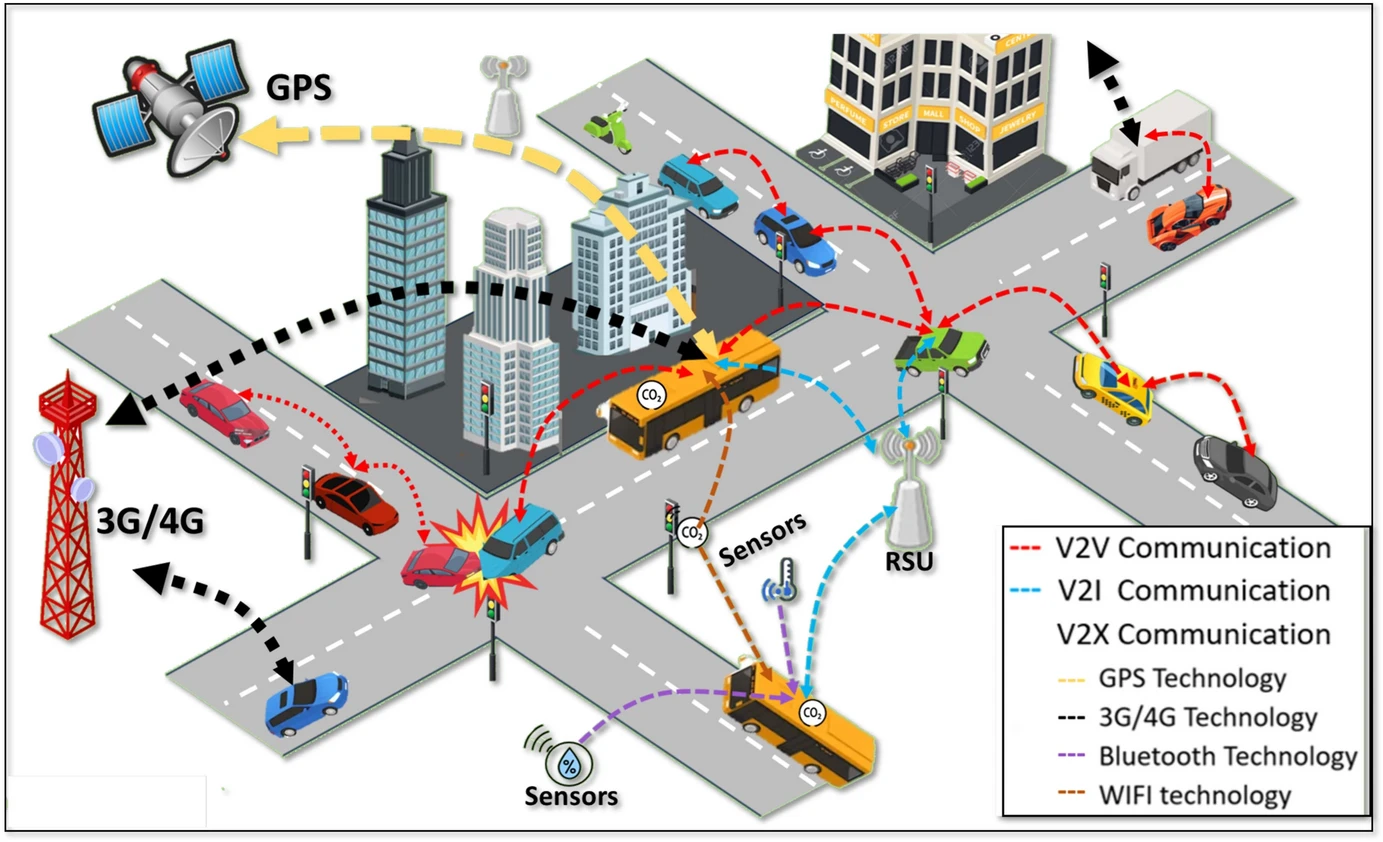
\includegraphics[width=0.9\textwidth]{VANET artitecture.png}
\caption{معماری شبکه اقتضایی خودرویی و انواع ارتباطات خودرو با هر موجودیت}
\label{fig:vanet_arch}
\end{figure}

شکل \ref{fig:vanet_arch} معماری کلی شبکه اقتضایی خودرویی و انواع ارتباطات خودرو با هر موجودیت \LTRfootnote{\lr{Vehicle-to-Everything (V2X)}} از جمله ارتباط خودرو به خودرو \LTRfootnote{\lr{Vehicle-to-Vehicle (V2V)}}، خودرو به زیرساخت \LTRfootnote{\lr{Vehicle-to-Infrastructure (V2I)}}، خودرو به عابر پیاده \LTRfootnote{\lr{Vehicle-to-Pedestrian (V2P)}}، خودرو به ابر \LTRfootnote{\lr{Vehicle-to-Cloud (V2C)}} و خودرو به پهپاد \LTRfootnote{\lr{Vehicle-to-UAV (VTU)}} و خودرو به شبکه \LTRfootnote{\lr{Vehicle-to-Network (V2N)}} را نشان می‌دهد.

\subsection{ارکان اصلی شبکه اقتضایی خودرویی}

ارکان اصلی شبکه اقتضایی خودرویی عبارتند از:

\begin{itemize}
  \item \textbf{واحدهای سوارشونده \LTRfootnote{\lr{On-Board Unit (OBU)}}}: سخت‌افزارهایی که در هر خودرو نصب شده و امکان ارتباط با واحدهای کنارجاده‌ای و واحدهای سوارشونده دیگر را فراهم می‌کنند \cite{hozouriOverviewVANETVehicular2023}.
  \item \textbf{واحدهای کنارجاده‌ای \LTRfootnote{\lr{Road-Side Unit (RSU)}}}: واحدهای ثابتی که در کنار جاده‌ها نصب شده و ارتباط خودروها با زیرساخت را برقرار می‌کنند \cite{hozouriOverviewVANETVehicular2023}.
  \item \textbf{مرجع قابل اعتماد \LTRfootnote{\lr{Trusted Authority (TA)}}}: مرجع مرکزی مسئول مدیریت امنیت و صدور اعتبارنامه‌ها \cite{rahmawatiagustinaSystematicLiteratureReview2025}.
\end{itemize}

\subsection{اهمیت  شبکه اقتضایی خودرویی}

اهمیت  شبکه اقتضایی خودرویی از جنبه‌های مختلفی قابل بررسی است:

\begin{itemize}
  \item \textbf{ایمنی ترافیک:} ارائه هشدارهای ایمنی بلادرنگ مانند هشدار تصادف جلو، هشدار تغییر لاین و هشدار شرایط جاده \cite{hozouriOverviewVANETVehicular2023}.
  \item \textbf{بهینه‌سازی ترافیک:} مدیریت هوشمند تقاطع‌ها، کاهش ازدحام و بهبود جریان ترافیک \cite{xuInternetVehiclesBig2018}.
  \item \textbf{سرویس‌های اطلاعاتی:} ارائه اطلاعات ناوبری، شرایط آب‌وهوایی و سرویس‌های سرگرمی \cite{hozouriOverviewVANETVehicular2023}.
  \item \textbf{خودروهای خودران:} پشتیبانی از رانندگی خودکار از طریق تبادل اطلاعات بلادرنگ \cite{xuInternetVehiclesBig2018}.
\end{itemize}

\subsection{ویژگی‌های متمایز  شبکه اقتضایی خودرویی}

 شبکه اقتضایی خودرویی ویژگی‌های منحصربفردی دارند که آن‌ها را از سایر شبکه‌های بی‌سیم متمایز می‌سازد \cite{hozouriOverviewVANETVehicular2023}:

\begin{itemize}
  \item \textbf{تحرک بالا:} گره‌ها می‌توانند سرعت‌های بالایی داشته باشند.
  \item \textbf{تغییرات مکرر توپولوژی:} ساختار شبکه به طور مداوم تغییر می‌کند.
  \item \textbf{منابع محاسباتی نامحدود:} برخلاف شبکه‌های حسگر، خودروها محدودیت انرژی ندارند.
  \item \textbf{تأخیر کم:} ارتباطات بلادرنگ برای سرویس‌های ایمنی ضروری است.
  \item \textbf{امنیت داده‌ها:} داده‌ها باید رمزنگاری شده و از تغییر محافظت شوند.
\end{itemize}

% ========================================================================
% فصل سوم: محدودیت‌ها و چالش‌ها
% ========================================================================
\section{محدودیت‌ها و چالش‌ها}

\subsection{چالش‌های شبکه‌سازی}

 شبکه اقتضایی خودرویی با چالش‌های متعددی در حوزه شبکه‌سازی مواجه هستند \cite{hozouriOverviewVANETVehicular2023}:

\begin{itemize}
  \item \textbf{تکه‌تکه شدن مکرر شبکه:} تراکم و تحرک بالای گره‌ها باعث قطع و وصل مکرر اتصالات می‌شود.
  \item \textbf{مشکلات مسیریابی:} یافتن مسیر مناسب برای ارسال پیام‌ها در شبکه‌های پویا دشوار است.
  \item \textbf{کمبود طیف فرکانسی:} استاندارد خودرو به شبکه و ابر \LTRfootnote{\lr{DSRC}} دارای مشکلات قابلیت اطمینان و مقیاس‌پذیری است.
  \item \textbf{تأثیرات محیطی:} ساختمان‌ها، خودروها و درختان می‌توانند سیگنال‌ها را مختل کنند.
\end{itemize}

\subsection{چالش‌های مدیریت منابع}

مدیریت منابع در  شبکه اقتضایی خودرویی با چالش‌های زیر مواجه است \cite{hozouriOverviewVANETVehicular2023, niSecuringFogComputing2018}:

\begin{itemize}
  \item \textbf{منابع مشترک:} کانال‌های پهنای باند و واحدهای کنارجاده‌ای منابع مشترکی هستند که باید بهینه مدیریت شوند.
  \item \textbf{تخصیص منابع رادیویی:} تکنیک‌های کنترل دسترسی رسانه \LTRfootnote{\lr{MAC}} برای تضمین دسترسی عادلانه به کانال ضروری هستند.
  \item \textbf{هزینه استقرار:} استقرار زیرساخت  شبکه اقتضایی خودرویی نیازمند سرمایه‌گذاری قابل توجهی است.
\end{itemize}

\subsection{چالش‌های مقیاس‌پذیری}

مقیاس‌پذیری یکی از مهمترین چالش‌های  شبکه اقتضایی خودرویی است \cite{xuInternetVehiclesBig2018}:

\begin{itemize}
  \item افزایش تعداد خودروهای متصل نیازمند مدیریت حجم عظیمی از داده‌ها است.
  \item حجم داده‌های تولید شده توسط خودروهای هوشمند به هزاران گیگابایت در روز می‌رسد.
  \item پردازش بلادرنگ این حجم از داده‌ها نیازمند منابع محاسباتی قابل توجهی است.
\end{itemize}

\subsection{چالش‌های استانداردسازی}

عدم وجود استانداردهای یکپارچه یکی دیگر از چالش‌های مهم است \cite{farsimadanReviewSecurityChallenges2025}:

\begin{itemize}
  \item تنوع فناوری‌های ارتباطی \lr{(DSRC, LTE, 5G)} و نیاز به سازگاری بین آنها
  \item نیاز به استانداردهای مشترک برای تبادل پیام‌ها و تصدیق هویت
  \item چالش‌های بین‌المللی در یکپارچه‌سازی سیستم‌های مختلف
\end{itemize}

% ========================================================================
% فصل چهارم: مشکلات امنیتی
% ========================================================================
\section{مشکلات امنیتی}

\subsection{الگوی تهدید}

 شبکه اقتضایی خودرویی در برابر حملات امنیتی مختلفی آسیب‌پذیر هستند. بر اساس مطالعات انجام شد تحلیل تهدیدات و معماری امنیتی  شبکه اقتضایی خودرویی نشان می‌دهد که حفظ تعادل بین کاهش مؤثر تهدیدات و حداقل تأثیر بر عملکرد سیستم از اهمیت بالایی برخوردار است \cite{SecuringVehicularAd,farsimadanReviewSecurityChallenges2025, VanetSecurityPrivacy, linGSISSecurePrivacyPreserving2007}.

\subsection{حملات بر زیرساخت}

\begin{itemize}
  \item \textbf{حملات منع سرویس:} اشباع واحدهای کنارجاده‌ای با اطلاعات اضافی برای جلوگیری از عملکرد صحیح
  \item \textbf{تقلید هویت:} مهاجمان خود را به جای واحدهای سوارشونده یا واحدهای کنارجاده‌ای جا می‌زنند
  \item \textbf{استراق سمع:} دسترسی غیرمجاز به اطلاعات خصوصی
\end{itemize}

\subsection{حملات بر حریم خصوصی}

\begin{itemize}
  \item \textbf{افشای هویت:} نقض اطلاعات هویتی سرنشینان خودرو
  \item \textbf{ردیابی موقعیت:} ردیابی موقعیت و مسیر خودرو توسط مهاجم
\end{itemize}

\subsection{حملات بر اعتماد داده}

\begin{itemize}
  \item \textbf{دستکاری پیام:} تغییر، حذف یا اصلاح داده‌ها در حین انتقال
  \item \textbf{حملات جعل:} تولید اطلاعات نادرست یا جعلی
  \item \textbf{حملات سیبل:} ایجاد هویت‌های متعدد توسط یک گره
\end{itemize}

\subsection{الزامات امنیتی}

برای تضمین امنیت  شبکه اقتضایی خودرویی، الزامات زیر باید برآورده شوند \cite{farsimadanReviewSecurityChallenges2025, VanetSecurityPrivacy}:

\begin{itemize}
\item \textbf{دسترسی:} ارتباطات باید به موقع در دسترس گیرندگان مورد نظر باشند
\item \textbf{محرمانگی:} داده‌ها باید رمزنگاری و محافظت شوند
\item \textbf{تصدیق:} هویت تمایز بین اشیاء معتبر و عناصر مخرب
\item \textbf{یکپارچگی:} داده‌ها باید به موقع تأیید شوند
\item \textbf{حریم:} خصوصی محافظت از اطلاعات شخصی کاربران
\item \textbf{اعتماد:} اطمینان بین موجودیت‌ها برای انتقال امن داده‌ها
\end{itemize}


یکی از راهکارها برای تضمین امنیت در شبکه اقتضایی خودرویی، استفاده از سیستم‌های تصدیق اصالت پیام مبتنی بر واحدهای کنارجاده‌ای است. طرح \lr{RAISE} با استفاده از واحدهای کنارجاده‌ای برای تأیید اصالت پیام‌های ارسالی از خودروها و اطلاع‌رسانی نتایج به خودروها، عملکرد بهتری نسبت به روش‌های قبلی از نظر نسبت از دست رفتن پیام و تأخیر ارائه می‌دهد \cite{zhangRAISEEfficientRSUAided2008}. همچنین، این طرح از رویکرد \lr{k-anonymity} برای حفاظت از حریم خصوصی هویت کاربر استفاده می‌کند، به طوری که یک مهاجم نمی‌تواند یک پیام خاص را با یک خودروی معین مرتبط کند \cite{zhangRAISEEfficientRSUAided2008}.

\subsection{نقش هوش مصنوعی در تقویت امنیت}

روش‌های هوش مصنوعی و یادگیری ماشین نقش مهمی در تقویت امنیت  شبکه اقتضایی خودرویی ایفا می‌کنند \cite{farsimadanReviewSecurityChallenges2025}:

\begin{itemize}
  \item \textbf{تشخیص ناهنجاری:} استفاده از شبکه‌های عصبی \lr{CNN} و \lr{LSTM} برای شناسایی رفتارهای غیرعادی
  \item \textbf{تشخیص حملات بی‌سیم:} استفاده از یادگیری بدون نظارت برای شناسایی حملات پارازیتی
  \item \textbf{تشخیص حملات اتومبیل:} استفاده از یادگیری بدون نظارت برای شناسایی حملات بر شبکه داخلی اتومبیل
  \item \textbf{تشخیص آسیب‌پذیری:} تحلیل ترافیک شبکه زنده برای شناسایی آسیب‌پذیری‌ها
  \item \textbf{یادگیری فدرال:} ترکیب بلاکچین و یادگیری فدرال برای انتقال اطلاعات امن با حفظ حریم خصوصی
  \item \textbf{منطق فازی:} محاسبه اعتماد برای دقت و یکپارچگی پیام‌های رویداد
  \item \textbf{یادگیری تقویتی:} ارزیابی قابلیت اطمینان خودروهای رانندگی خودکار
\end{itemize}

% ========================================================================
% فصل پنجم: مروری بر بلاکچین
% ========================================================================
\section{مرور کلی بر بلاکچین}

\subsection{تعریف و مفهوم}

بلاکچین\LTRfootnote{\lr{blockchain}} یک دفتر کل دیجیتال غیرمتمرکز و توزیع‌شده است که تراکنش‌ها را به صورت ایمن و شفاف ثبت می‌کند \cite{razaBlockchainBasedReputationTrust2024, hozouriOverviewVANETVehicular2023}. هر بلوک شامل هش بلوک قبلی است که زنجیره‌ای از بلوک‌ها را ایجاد می‌کند \cite{razaBlockchainBasedReputationTrust2024}.

\subsection{لایه‌های بلاکچین}

معماری بلاکچین از شش لایه اصلی تشکیل شده است \cite{razaBlockchainBasedReputationTrust2024}:

\begin{enumerate}
  \item \textbf{لایه داده:} ساختار بلوک‌ها و تراکنش‌ها
  \item \textbf{لایه شبکه:} ارتباطات همتا به همتا
  \item \textbf{لایه اجماع:} مکانیزم‌های تأیید تراکنش‌ها
  \item \textbf{لایه انگیزش:} پاداش‌ها و مشوق‌ها
  \item \textbf{لایه قرارداد:} قراردادهای هوشمند
  \item \textbf{لایه کاربرد:} برنامه‌های کاربردی
\end{enumerate}

\begin{figure}[H]
\centering
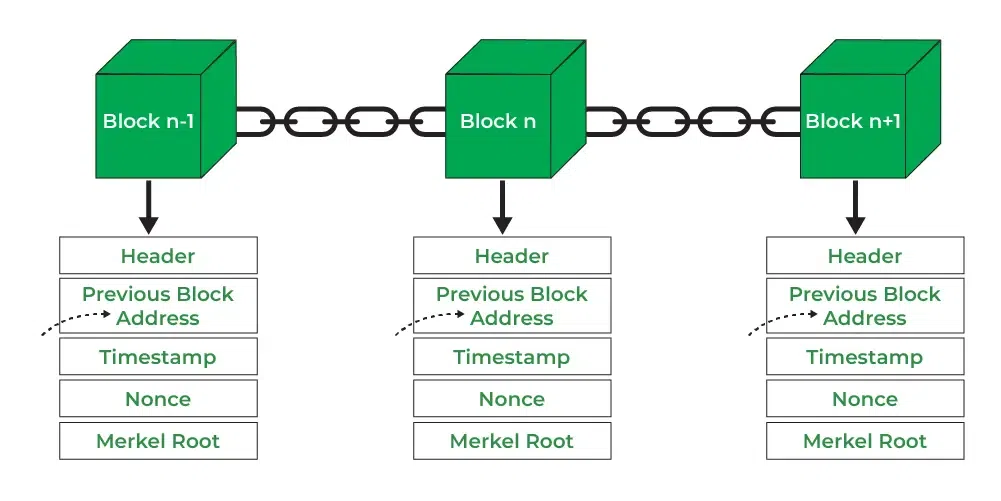
\includegraphics[width=0.8\textwidth]{blockchainstruct1.png}
\caption{ساختار عمومی بلاکچین: زنجیره‌ای از بلوک‌ها با اتصال هش هر بلوک به بلوک قبلی}
\label{fig:blockchain_struct}
\end{figure}

شکل \ref{fig:blockchain_struct} ساختار عمومی بلاکچین و نحوه اتصال هر بلوک با هش بلوک قبلی را نشان می‌دهد.

\subsection{مکانیزم‌های اجماع}

مکانیزم‌های اجماع نقش حیاتی در عملکرد بلاکچین ایفا می‌کنند \cite{razaBlockchainBasedReputationTrust2024}:

\begin{table}[H]
\centering
\caption{مکانیزم‌های اجماع در بلاکچین}
\label{tab:consensus}
\begin{tabular}{p{2.5cm} p{4cm} p{2.5cm} p{2.5cm}}
\toprule
\textbf{الگوریتم} & \textbf{ویژگی کلیدی} & \textbf{مصرف انرژی} & \textbf{مقیاس‌پذیری} \\
\midrule
\lr{PoW} & پازل محاسباتی & بسیار بالا & پایین \\
\lr{PoS} & مبتنی بر سهام اقتصادی & پایین & متوسط \\
\lr{DPoS} & رأی‌دهی به ازای هر سهم & پایین & بالا \\
\lr{PBFT} & پیچیدگی چندجمله‌ای & پایین & متوسط \\
\bottomrule
\end{tabular}
\end{table}

\subsection{چالش‌های بلاکچین}

فناوری بلاکچین با چالش‌های متعددی مواجه است \cite{razaBlockchainBasedReputationTrust2024}:

\begin{itemize}
  \item \textbf{پیچیدگی طراحی:} ساختار پیچیده بلاکچین
  \item \textbf{حریم خصوصی و امنیت:} حملات ۵۱ درصد، مشکلات کیف پول
  \item \textbf{پروتکل اجماع:} توازن بین امنیت، مقیاس‌پذیری و کارایی انرژی
  \item \textbf{همکاری‌پذیری:} ادغام با سیستم‌های موجود
  \item \textbf{مشکل مقیاس‌پذیری:} محدودیت در تعداد تراکنش‌ها در ثانیه
  \item \textbf{مصرف انرژی:} هزینه بالای محاسبات
\end{itemize}

% ========================================================================
% فصل ششم: بلاکچین به عنوان راه حل
% ========================================================================
\section{بلاکچین یک راه حل خوب}

\subsection{مزایای بلاکچین در  شبکه اقتضایی خودرویی}

بلاکچین با ویژگی‌های منحصربفرد خود می‌تواند بسیاری از مشکلات  شبکه اقتضایی خودرویی را حل کند \cite{razaBlockchainBasedReputationTrust2024, fengBPASBlockchainAssistedPrivacyPreserving2020, ghovanlooyghajarSBTMSScalableBlockchain2021}:

\begin{itemize}
  \item \textbf{غیرمتمرکزسازی:} حذف نقطه شکست واحد و افزایش امنیت و تاب‌آوری
  \item \textbf{تغییرناپذیری:} داده‌ها قابل تغییر یا دستکاری نیستند
  \item \textbf{ردیابی:} جلوگیری از استفاده نادرست از داده‌ها از طریق تاریخچه کامل تراکنش‌ها
  \item \textbf{شفافیت:} ثبت شفاف تراکنش‌ها
  \item \textbf{قراردادهای هوشمند:} اجرای خودکار سیاست‌های امنیتی
\end{itemize}

\subsection{کاربردهای بلاکچین در شبکه اقتضایی خودرویی}

بلاکچین در حوزه‌های مختلف  شبکه اقتضایی خودرویی کاربرد دارد \cite{razaBlockchainBasedReputationTrust2024, hozouriOverviewVANETVehicular2023}:

\begin{itemize}
  \item \textbf{افزایش امنیت:} تعیین صحت پیام‌های پخش شده بین خودروها
  \item \textbf{حریم خصوصی:} رمزنگاری کلید عمومی برای محافظت از داده‌های حساس
  \item \textbf{مدیریت اعتماد:} ذخیره مقادیر اعتماد در بلاکچین
  \item \textbf{مدیریت هویت:} مدیریت غیرمتمرکز کلیدها و گواهی‌نامه‌ها
  \item \textbf{ ردیابی خودرو:} جلوگیری از دستکاری کیلومترشمار
\end{itemize}

\subsection{مدل‌های مدیریت اعتماد}

بلاکچین امکان ایجاد مدل‌های مدیریت اعتماد غیرمتمرکز را فراهم می‌کند \cite{razaBlockchainBasedReputationTrust2024, ghovanlooyghajarSBTMSScalableBlockchain2021}:

\begin{itemize}
  \item \textbf{اعتماد مبتنی بر توصیه:} بر اساس توصیه‌های عناصر دیگر
  \item \textbf{اعتماد مبتنی بر پیش‌بینی:} بر اساس الگوهای رفتاری
  \item \textbf{اعتماد مبتنی بر شهرت:} بر اساس سابقه عملکرد
  \item \textbf{اعتماد مبتنی بر سیاست:} بر اساس قوانین و مقررات
\end{itemize}

% ========================================================================
% فصل هفتم: مشکلات بلاکچین و راه حل‌ها
% ========================================================================
\section{مشکلات بلاکچین و راهکارها}

\subsection{محدودیت‌های بلاکچین}

علی‌رغم مزایای فراوان، بلاکچین‌های سنتی محدودیت‌هایی در حوزه  شبکه اقتضایی خودرویی دارند \cite{razaBlockchainBasedReputationTrust2024, IOTATANGLE20}:

\begin{itemize}
  \item \textbf{مقیاس‌پذیری پایین:} تعداد محدود تراکنش‌ها در ثانیه (بیت‌کوین: ۷، اتریوم: ۱۵)
  \item \textbf{مصرف انرژی بالا:} الگوریتم اثبات کار نیازمند منابع محاسباتی قابل توجه
  \item \textbf{تأخیر بالا:} زمان تأیید تراکنش‌ها برای کاربردهای بلادرنگ مناسب نیست
  \item \textbf{هزینه تراکنش:} وجود کارمزد برای هر تراکنش
  \item \textbf{محدودیت ذخیره‌سازی:} حجم زیاد داده‌ها برای ذخیره‌سازی در بلاکچین
\end{itemize}

\subsection{راهکارهای موجود}

برای رفع محدودیت‌های بلاکچین در  شبکه اقتضایی خودرویی، راهکارهای مختلفی ارائه شده است \cite{ghovanlooyghajarSBTMSScalableBlockchain2021, razaBlockchainBasedReputationTrust2024}:

\begin{itemize}
  \item \textbf{شاردینگ:} تقسیم شبکه به بخش‌های کوچکتر برای افزایش مقیاس‌پذیری
  \item \textbf{الگوریتم‌های اجماع جایگزین:} استفاده از \lr{PoS}، \lr{DPoS} و \lr{PBFT} به جای \lr{PoW}
  \item \textbf{زنجیره‌های فرعی:} استفاده از زنجیره‌های فرعی برای کاهش بار شبکه اصلی
  \item \textbf{لایه‌های مقیاس‌پذیری:} استفاده از لایه‌های مقیاس‌پذیری مانند \lr{Lightning Network}
\end{itemize}

\subsection{سیستم مدیریت اعتماد مقیاس‌پذیر مبتنی بر بلاکچین \lr{(SBTMS)}}

سیستم \lr{SBTMS} یکی از راهکارهای نوین برای حل مشکلات بلاکچین در شبکه‌های اقتضایی خودرویی است \cite{ghovanlooyghajarSBTMSScalableBlockchain2021}:

\begin{itemize}
  \item \textbf{معماری غیرمتمرکز:} استفاده از بلاکچین برای ایجاد پلتفرم غیرمتمرکز
  \item \textbf{الگوریتم شاردینگ:} تقسیم شبکه به بخش‌های کوچکتر برای مقیاس‌پذیری
  \item \textbf{استنباط بیزی:} محاسبه اعتماد بر اساس فرمول‌های بیزی
  \item \textbf{پروتکل \lr{PBFT}:} پروتکل تحمل خطای بیزانس عملی
\end{itemize}

نتایج شبیه‌سازی \lr{SBTMS} نشان می‌دهد که الگوریتم شاردینگ زمان تولید بلوک را به صورت تقریباً خطی افزایش می‌دهد، در حالی که در الگوریتم \lr{PoW} این زمان به صورت نمایی افزایش می‌یابد \cite{ghovanlooyghajarSBTMSScalableBlockchain2021}.

% ========================================================================
% فصل هشتم: IOTA Tangle
% ========================================================================
\section{\lr{IOTA Tangle} چیست؟}

\subsection{مفهوم \lr{IOTA Tangle}}

\lr{IOTA Tangle} یک فناوری دفتر کل توزیع‌شده \LTRfootnote{\lr{DLT}} است که بر اساس ساختار گراف جهت‌دار بدون دور \LTRfootnote{\lr{DAG}} طراحی شده است \cite{IOTATANGLE20, silvanoIotaTangleCryptocurrency2020}. برخلاف بلاکچین‌های سنتی که از زنجیره بلوک‌ها استفاده می‌کنند، \lr{IOTA Tangle} از ساختار \lr{Tangle} استفاده می‌کند که در آن هر تراکنش جدید به دو تراکنش قبلی ارجاع می‌دهد \cite{silvanoIotaTangleCryptocurrency2020}.

\begin{figure}[H]
\centering
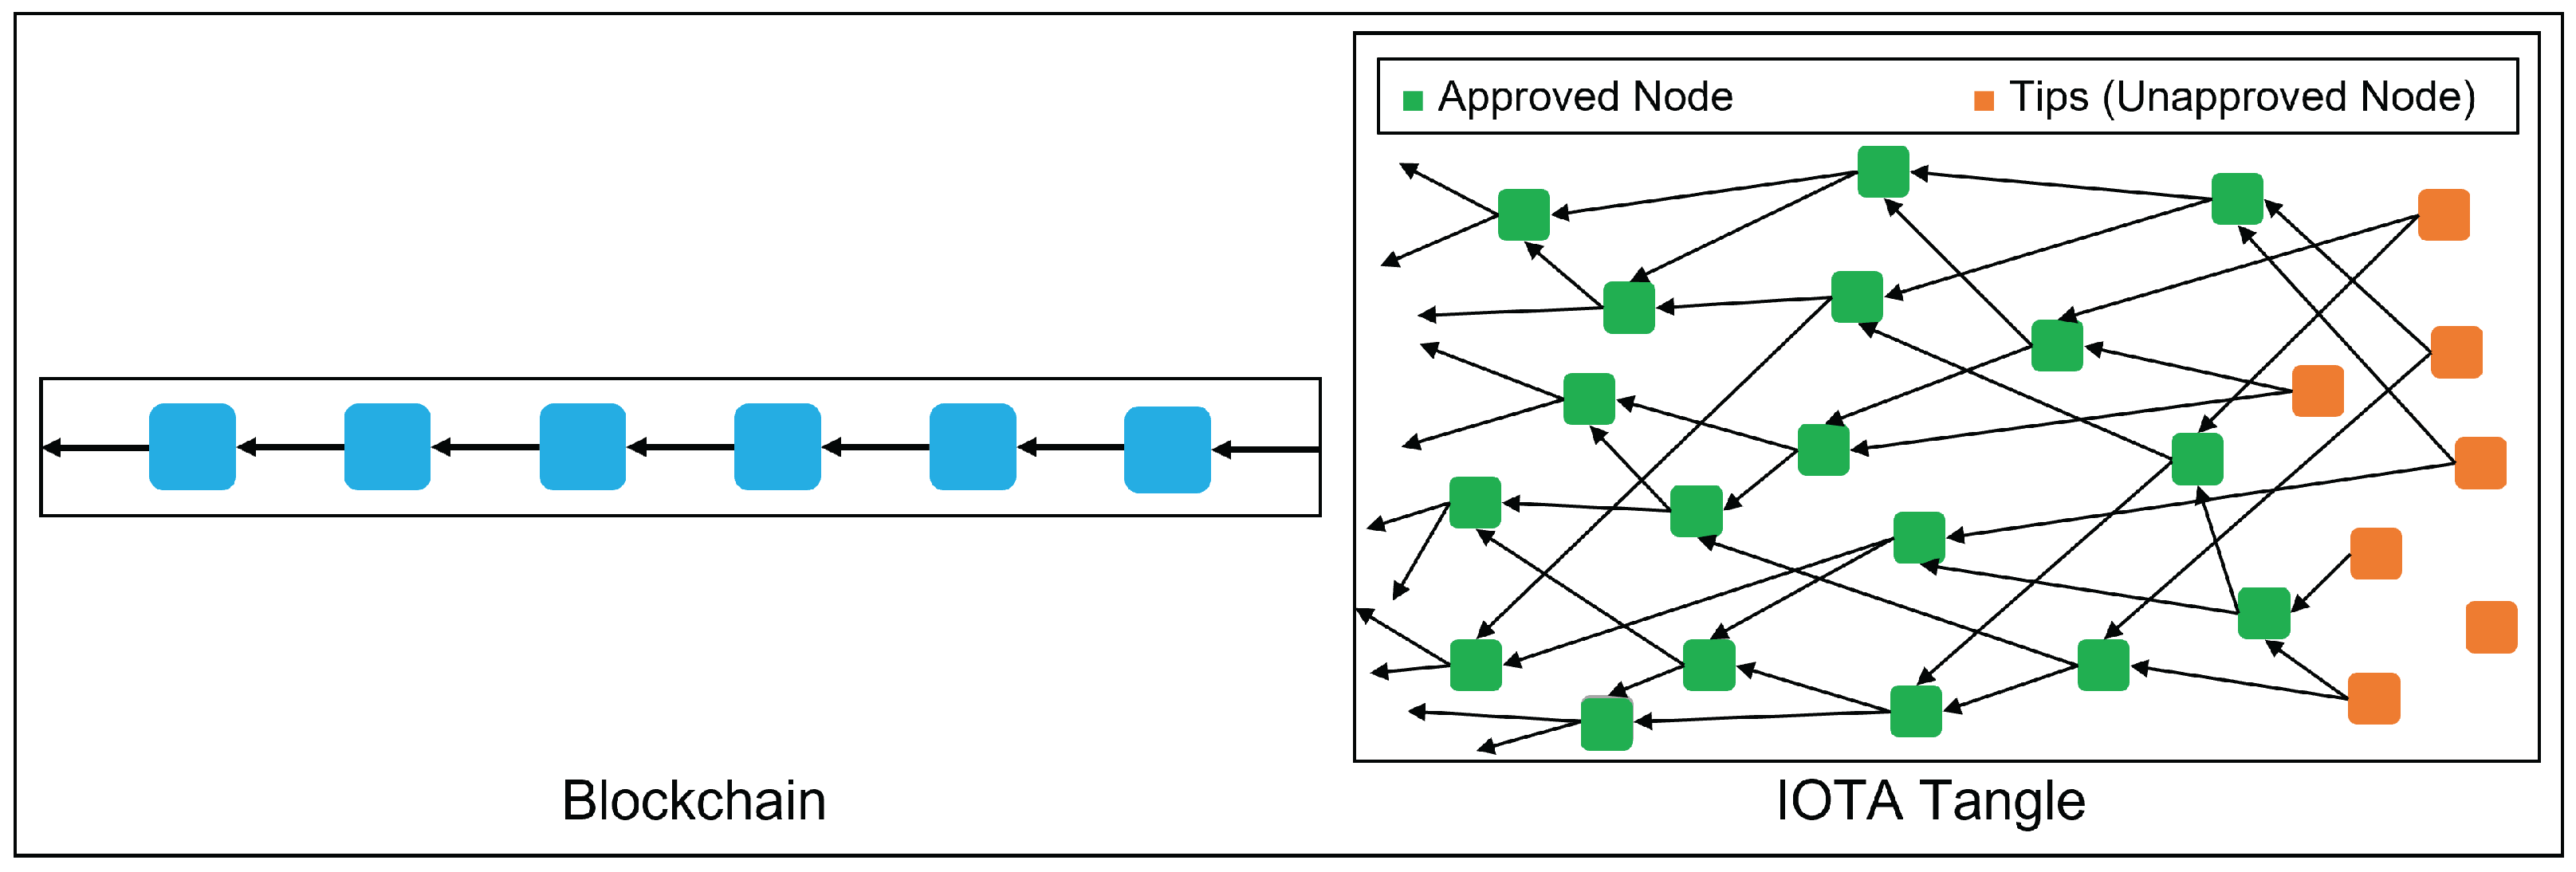
\includegraphics[width=0.95\textwidth]{IOTA vs Blockchain.png}
\caption{مقایسه تصویری \lr{IOTA Tangle} با بلاکچین سنتی}
\label{fig:iota_vs_bc}
\end{figure}

شکل \ref{fig:iota_vs_bc} مقایسه تصویری \lr{IOTA Tangle} با بلاکچین سنتی را نشان می‌دهد که بلاکچین به صورت یک زنجیر از بلوک ها پشت سر هم قرار گرفتن ولی درون \lr{IOTA Tangle} به صورت یک گراف جهت دار بدون دور کنار یکدیگر قرار گرفتند.

\subsection{ویژگی‌های کلیدی \lr{IOTA Tangle V2.0}}

\lr{IOTA Tangle V2.0} ویژگی‌های مهمی را ارائه می‌دهد \cite{IOTATANGLE20, sealeyIOTATangle202022}. این نسخه با حذف هماهنگ‌کننده متمرکز و معرفی پروتکل‌های جدید اجماع، به مقیاس‌پذیری و غیرمتمرکزسازی واقعی دست یافته است \cite{sealeyIOTATangle202022}:

\begin{itemize}
  \item \textbf{مقیاس‌پذیری بالا:} با افزایش تراکنش‌ها، شبکه قوی‌تر شده و تأییدها سریع‌تر انجام می‌شوند.
  \item \textbf{بدون کارمزد:} تراکنش‌ها بدون هیچ هزینه‌ای انجام می‌شوند.
  \item \textbf{اجماع غیرمتمرکز:} استفاده از پروتکل \lr{FPC}.
  \item \textbf{قراردادهای هوشمند:} پشتیبانی از قراردادهای هوشمند از طریق \lr{ISCP}.
  \item \textbf{امضای \lr{Ed25519}:} استفاده از طرح امضای کارآمد و ایمن.
\end{itemize}

\subsection{چگونگی رفع مشکلات}

\lr{IOTA Tangle} مشکلات اصلی بلاکچین در شبکه‌های اقتضایی خودرویی را به شرح زیر رفع می‌کند \cite{IOTATANGLE20, silvanoIotaTangleCryptocurrency2020}:

\begin{table}[H]
\centering
\caption{مقایسه \lr{IOTA Tangle} با بلاکچین}
\label{tab:iota_vs_bc}
\begin{tabular}{p{3.5cm} p{4.5cm} p{4.5cm}}
\toprule
\textbf{ویژگی} & \textbf{بلاکچین} & \textbf{\lr{IOTA Tangle}} \\
\midrule
ساختار & زنجیره بلوک‌ها & گراف جهت‌دار بدون دور \\
کارمزد & بالا & بدون کارمزد \\
\lr{TPS} & پایین (۷-۱۵) & بالا و مقیاس‌پذیر \\
مصرف انرژی & بالا & پایین \\
ماینر & نیاز دارد & نیاز ندارد \\
\bottomrule
\end{tabular}
\end{table}

\subsection{معماری \lr{IOTA Tangle V2.0}}

معماری پروتکل \lr{IOTA  Tangle V2.0} از سه لایه اصلی تشکیل شده است \cite{IOTATANGLE20}:

\begin{enumerate}
  \item \textbf{لایه شبکه:} مدیریت عملیات سطح بایت و مبادلات همتا به همتا
  \item \textbf{لایه ارتباطات:} مدیریت پیام‌ها، انتخاب نکات و کنترل نرخ
  \item \textbf{لایه کاربردی:} اجرای بارهای پیام و اجرای اجماع
\end{enumerate}

\subsection{کاربرد \lr{IOTA Tangle} در  شبکه اقتضایی خودرویی}

\lr{IOTA Tangle} در  شبکه اقتضایی خودرویی کاربردهای زیر را دارد \cite{feraudoDIVADIDbasedReputation2024, silvanoIotaTangleCryptocurrency2020}:

\begin{itemize}
  \item \textbf{ذخیره‌سازی امتیازات شهرت:} ذخیره ایمن امتیازات شهرت خودروها
  \item \textbf{تراکنش‌های بدون کارمزد:} امکان تبادل اطلاعات بدون هزینه
  \item \textbf{تأیید سریع:} تأیید سریع تراکنش‌ها برای کاربردهای بلادرنگ
  \item \textbf{امنیت سخت‌افزاری:} استفاده از امضای \lr{Ed25519} برای امنیت بالا
\end{itemize}

% ========================================================================
% فصل نهم: مدیریت هویت و شبه‌نام
% ========================================================================
\section{هویت خودمختار}

\subsection{مدیریت هویت چیست؟}

مدیریت هویت فرآیند شناسایی، تصدیق هویت و مدیریت دسترسی کاربران به سیستم‌ها و سرویس‌ها است \cite{mazzocca2025survey}. در  شبکه اقتضایی خودرویی، مدیریت هویت نقش حیاتی در تضمین امنیت و حریم خصوصی ایفا می‌کند.

\subsection{تکامل مدیریت هویت}

مدیریت هویت در طول زمان تکامل یافته است \cite{mazzocca2025survey}:

\begin{enumerate}
  \item \textbf{هویت متمرکز (۱۹۸۸-۱۹۹۸):} کنترل مرکزی توسط یک مرجع واحد
  \item \textbf{هویت فدرالی (۱۹۹۸-۲۰۰۵):} ورود یکپارچه به سرویس‌های مختلف
  \item \textbf{هویت کاربرمحور (۲۰۰۵-۲۰۱۲):} مدیریت مستقل هویت توسط کاربر
  \item \textbf{هویت خودمختار (۲۰۱۲ تا کنون):} کنترل کامل کاربر بر داده‌های خود
\end{enumerate}

\subsection{شبه‌نام چیست؟}

شبه‌نام\LTRfootnote{\lr{Pseudonym}} یک شناسه موقت و غیرقابل پیوند است که به جای هویت واقعی استفاده می‌شود \cite{rahmawatiagustinaSystematicLiteratureReview2025, luPseudonymChangingSocial2012}. استفاده از شبه‌نام به خودروها امکان می‌دهد تا بدون افشای هویت واقعی خود در شبکه شرکت کنند.

\subsection{چرخه حیات شبه‌نام}

چرخه حیات شبه‌نام شامل مراحل زیر است \cite{rahmawatiagustinaSystematicLiteratureReview2025}:

\begin{enumerate}
  \item \textbf{صدور:} تولید نام‌های مستعار رمزنگاری شده ایمن
  \item \textbf{استفاده:} استفاده در ارتباطات \lr{V2V} و \lr{V2I}
  \item \textbf{تغییر:} تغییر دوره‌ای شبه‌نام برای جلوگیری از ردیابی
  \item \textbf{حل:} شناسایی هویت واقعی توسط مراجع قانونی
  \item \textbf{لغو:} مسدود کردن خودروهای مخرب
\end{enumerate}

بر اساس مطالعات انجام شده، فقط ۱۲ درصد از طرح‌ها تمام مراحل چرخه حیات شبه‌نام را پیاده‌سازی کرده‌اند \cite{rahmawatiagustinaSystematicLiteratureReview2025}.

\subsection{هویت خودمختار چیست و چرا مطرح شده است؟}

هویت خودمختار یک رویکرد نوین در مدیریت هویت است که به کاربران کنترل کامل بر داده‌های شخصی خود را می‌دهد \cite{mazzocca2025survey}. هویت خودمختار بر اساس فناوری‌های دفتر کل توزیع‌شده، شناسه‌های غیرمتمرکز و اعتبارنامه‌های تأییدپذیر ساخته شده است.

\begin{figure}[H]
\centering
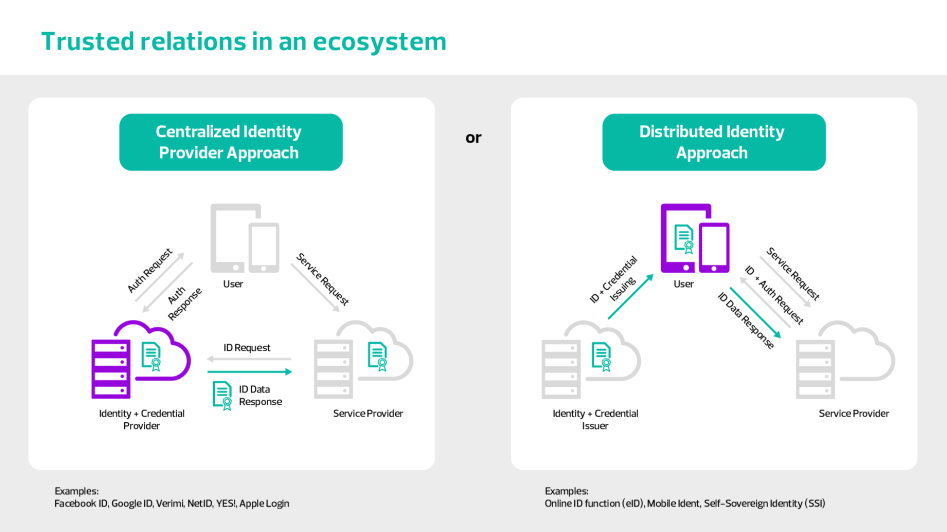
\includegraphics[width=0.85\textwidth]{SSI vs centeralized.png}
\caption{مقایسه معماری مدیریت هویت متمرکز و هویت خودمختار}
\label{fig:ssi_vs_centralized}
\end{figure}

شکل \ref{fig:ssi_vs_centralized} تفاوت معماری مدیریت هویت متمرکز و هویت خودمختار را نشان می‌دهد.

دلایل مطرح شدن هویت خودمختار عبارتند از:

\begin{itemize}
  \item \textbf{نقطه شکست واحد:} سیستم‌های متمرکز در برابر حملات آسیب‌پذیر هستند
  \item \textbf{نقض حریم خصوصی:} نقض داده‌ها در سیستم‌های متمرکز رایج است
  \item \textbf{کنترل محدود کاربر:} کاربران کنترل محدودی بر داده‌های خود دارند
  \item \textbf{نیاز به حریم خصوصی:} افزایش نگرانی‌ها در مورد حریم خصوصی داده‌ها
\end{itemize}

\subsection{شناسه‌های غیرمتمرکز چیست و چرا مطرح شده است؟}

شناسه‌های غیرمتمرکز شناسه‌های جهانی منحصربفردی هستند که بدون نیاز به مرجع مرکزی عمل می‌کنند \cite{mazzocca2025survey}. مثال:
\begin{center}
\texttt{\lr{did:example:123456789abcdefghi}}
\end{center}

\subsubsection{معماری شناسه‌های غیرمتمرکز}

معماری شناسه‌های غیرمتمرکز شامل اجزای زیر است \cite{mazzocca2025survey}:

\begin{itemize}
  \item \textbf{شناسه غیرمتمرکز:} شناسه جهانی منحصربفرد
  \item \textbf{سند شناسه غیرمتمرکز:} سند \lr{JSON-LD} حاوی کلیدهای عمومی و نقاط اتصال سرویس
  \item \textbf{روش شناسه غیرمتمرکز:} مشخص کننده نحوه ایجاد، حل، به‌روزرسانی و غیرفعال کردن شناسه غیرمتمرکز
  \item \textbf{ثبات داده تأییدپذیر:} مخزن ذخیره‌سازی اسناد شناسه غیرمتمرکز
\end{itemize}

\subsubsection{انواع شناسه‌های غیرمتمرکز}

\begin{itemize}
  \item \textbf{شناسه‌های غیرمتمرکز بی‌طرفه \LTRfootnote{Anywise}:} قابل استفاده با طرف‌های نامشخص
  \item \textbf{شناسه‌های غیرمتمرکز دو طرفه\LTRfootnote{Pairwise}:} فقط توسط شخص و یک طرف دیگر شناخته شده
  \item \textbf{شناسه‌های غیرمتمرکز چند طرفه \LTRfootnote{N-wise}:} توسط دقیقاً \lr{N} طرف شناخته شده
\end{itemize}

\begin{figure}[H]
\centering
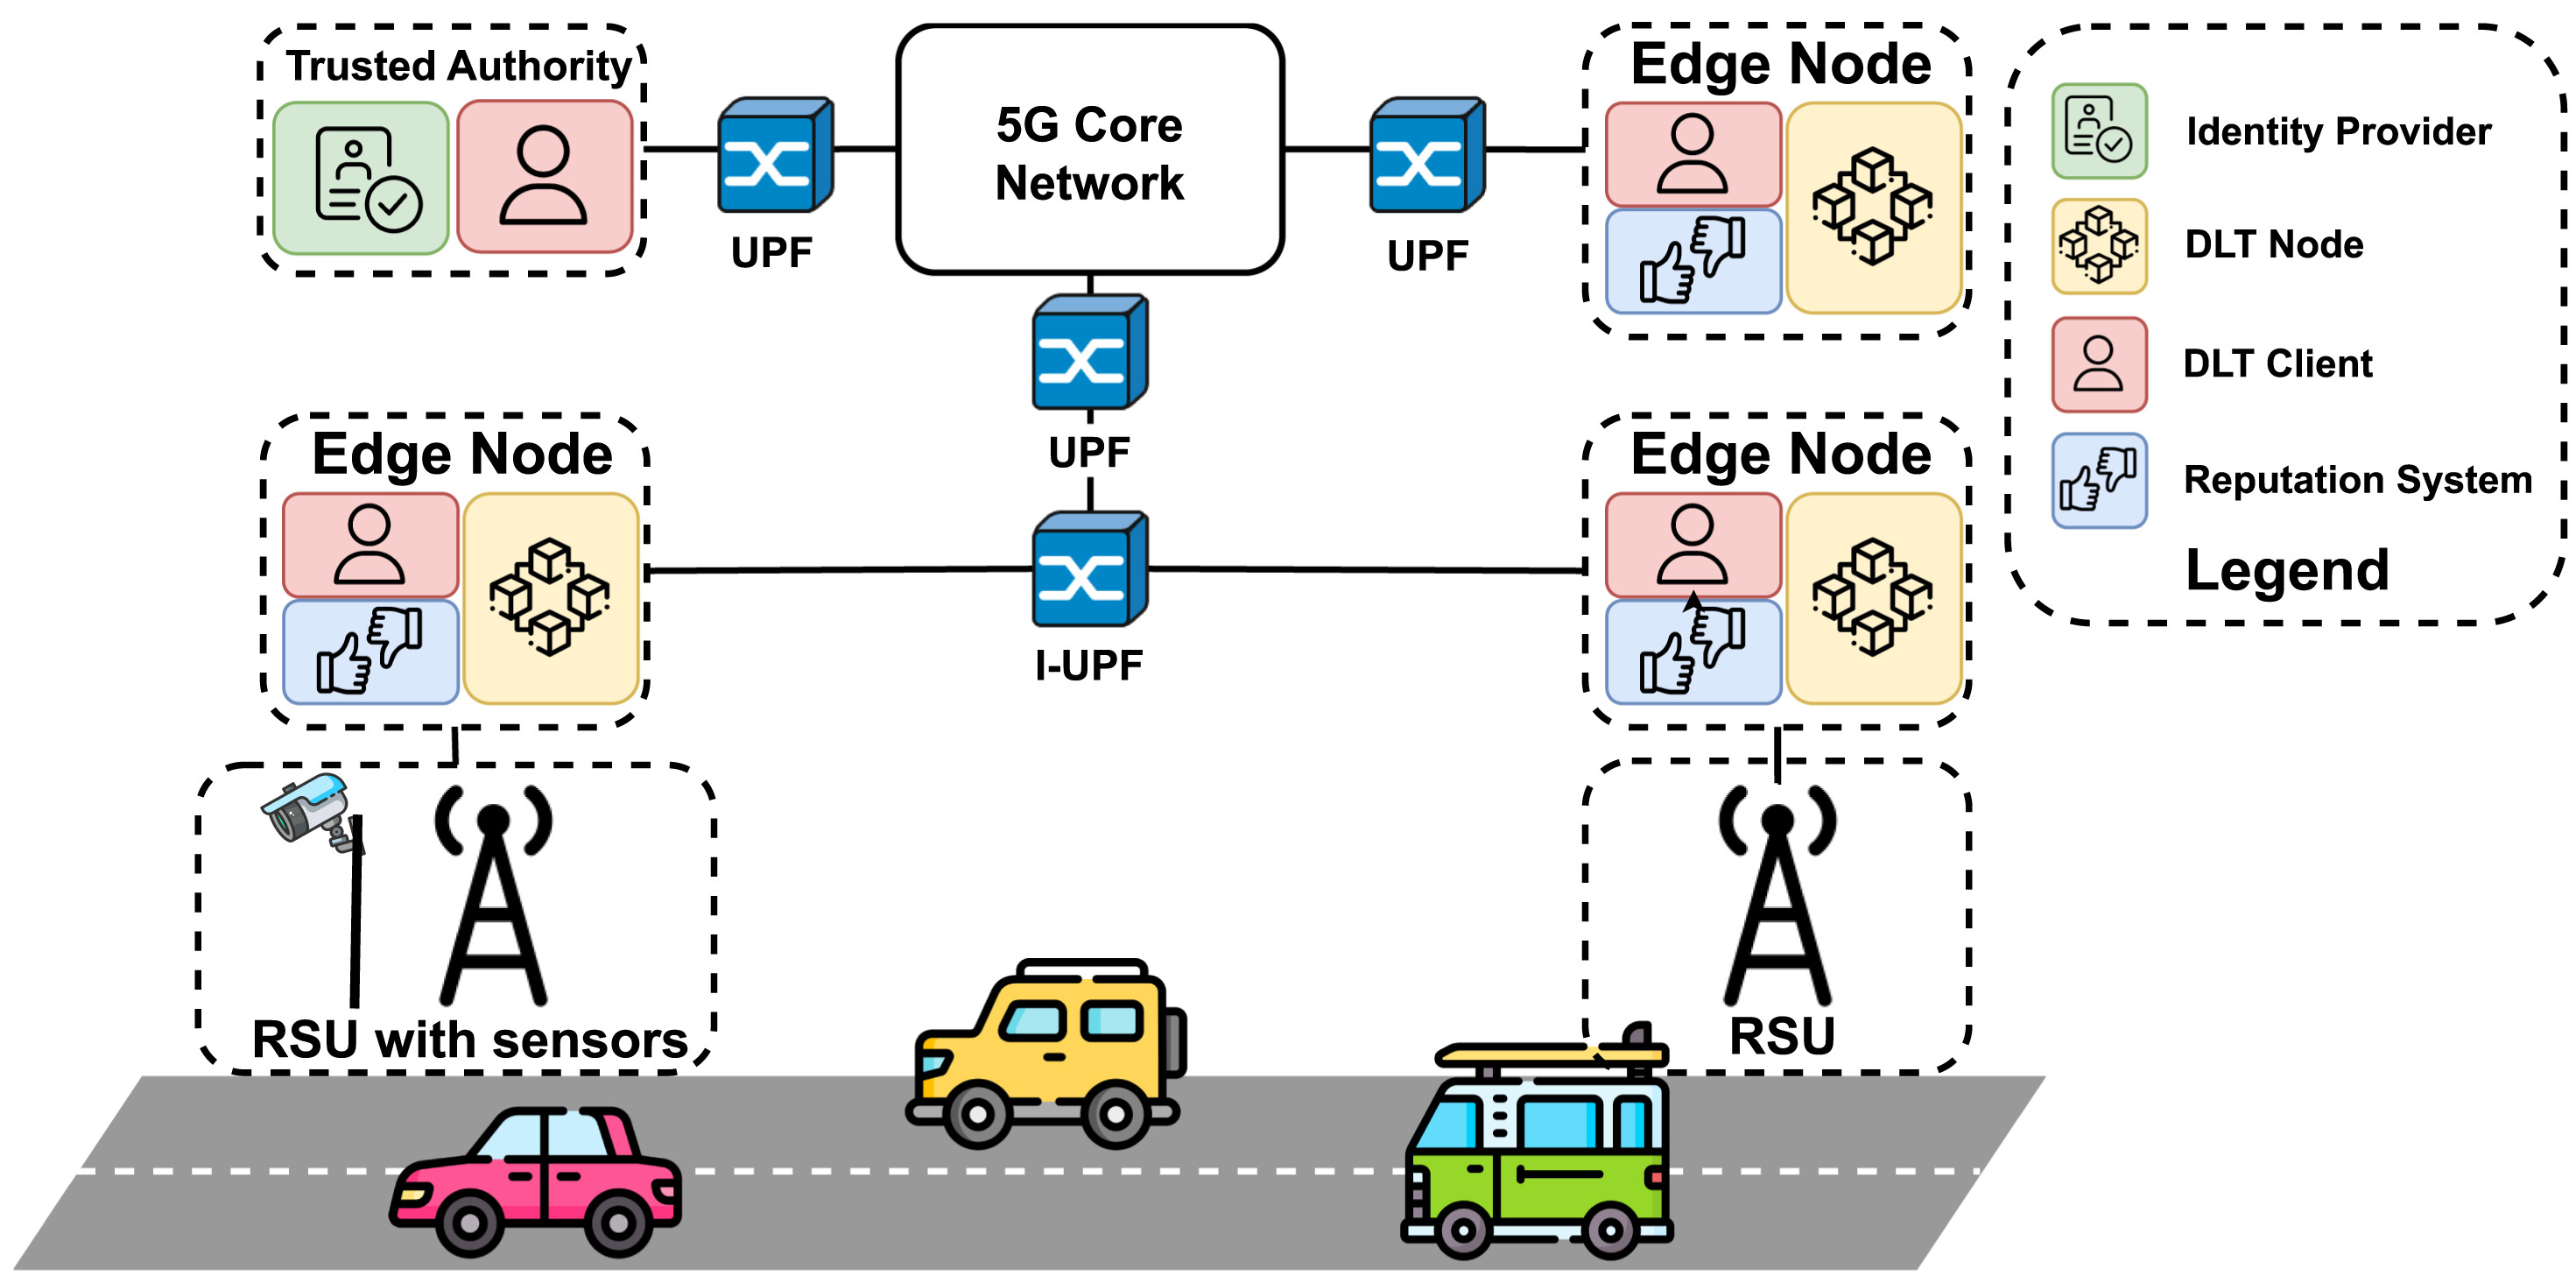
\includegraphics[width=0.9\textwidth]{DIVA.jpg}
\caption{معماری سیستم \lr{DIVA}: سیستم شهرت مبتنی بر شناسه‌های غیرمتمرکز برای انتقال امن در  شبکه اقتضایی خودرویی با استفاده از \lr{IOTA Tangle}}
\label{fig:diva_arch}
\end{figure}

شکل \ref{fig:diva_arch} معماری سیستم \lr{DIVA} را نشان می‌دهد که از شناسه‌های غیرمتمرکز برای شناسایی خودروها و \lr{IOTA Tangle} برای ذخیره ایمن امتیازات شهرت استفاده می‌کند. در این سیستم، خودروها با استفاده از شناسه‌های غیرمتمرکز شناسایی شده و امتیازات شهرت آنها بر اساس پیام‌های ایمنی و غیرایمنی محاسبه می‌شود \cite{feraudoDIVADIDbasedReputation2024}.

\subsection{اعتبارنامه‌های تأییدپذیر}

اعتبارنامه‌های تأییدپذیر مدارک الکترونیکی رمزنگاری شده و تغییرناپذیر هستند که توسط \lr{W3C} استانداردسازی شده‌اند \cite{mazzocca2025survey}.

بازیگران اصلی اعتبارنامه‌های تأییدپذیر عبارتند از:

\begin{itemize}
  \item \textbf{نگهدارنده\LTRfootnote{Holder}:} موجودیتی که اعتبارنامه تأییدپذیر را کنترل می‌کند
  \item \textbf{صادرکننده\LTRfootnote{Issuer}:} نهاد معتبری که اعتبارنامه تأییدپذیر را صادر می‌کند
  \item \textbf{تأییدکننده\LTRfootnote{Verifier}:} موجودیتی که به اعتبارنامه تأییدپذیر نیاز دارد
\end{itemize}

\subsection{چرا هویت خودمختار و شناسه‌های غیرمتمرکز در  شبکه اقتضایی خودرویی مطرح شده‌اند؟}

فناوری‌های هویت خودمختار و شناسه‌های غیرمتمرکز برای حل مشکلات امنیتی و حریم خصوصی در  شبکه اقتضایی خودرویی مطرح شده‌اند \cite{mazzocca2025survey, feraudoDIVADIDbasedReputation2024}:

\begin{itemize}
  \item \textbf{تصدیق هویت غیرمتمرکز:} حذف نیاز به مرجع مرکزی
  \item \textbf{حفظ حریم خصوصی:} استفاده از شناسه‌های غیرمتمرکز به عنوان شبه‌نام
  \item \textbf{قابلیت ردیابی شرطی:} امکان شناسایی هویت واقعی در صورت نیاز
  \item \textbf{مدیریت شهرت:} ذخیره امتیازات شهرت به صورت غیرمتمرکز
\end{itemize}

\subsection{مشکلات امنیتی رفع شده توسط شناسه‌های غیرمتمرکز و هویت خودمختار}

فناوری‌های شناسه‌های غیرمتمرکز و هویت خودمختار مشکلات زیر را در  شبکه اقتضایی خودرویی رفع می‌کنند \cite{mazzocca2025survey, feraudoDIVADIDbasedReputation2024}:

\begin{itemize}
  \item \textbf{نقطه شکست واحد:} حذف مرجع متمرکز با استفاده از شناسه‌های غیرمتمرکز
  \item \textbf{نقض حریم خصوصی:} استفاده از شناسه‌های غیرمتمرکز به عنوان شبه‌نام و افشاگری انتخابی
  \item \textbf{مدیریت گواهی‌نامه:} حذف نیاز به مدیریت گواهی‌نامه‌های پیچیده
  \item \textbf{حملات تقلید:} تصدیق هویت مبتنی بر رمزنگاری
  \item \textbf{حملات سیبل:} یک شناسه غیرمتمرکز برای هر خودرو
\end{itemize}

% ========================================================================
% فصل دهم: راهکارهای امنیتی
% ========================================================================
\section{طرح‌های موجود برای تصدیق هویت}

\subsection{حل مشکل شبه‌نام در  شبکه اقتضایی خودرویی}

شبه‌نام یکی از مهمترین چالش‌ها در حفظ حریم خصوصی  شبکه اقتضایی خودرویی است \cite{luPseudonymChangingSocial2012, al-aniPrivacySafetyImprovement2023, rahmawatiagustinaSystematicLiteratureReview2025}. راهکارهای موجود عبارتند از:

\subsubsection{تغییر شبه‌نام در نقاط اجتماعی (\lr{PCS})}

رویکرد \lr{PCS} پیشنهاد می‌کند که خودروها شبه‌نام خود را در نقاط اجتماعی تغییر دهند \cite{luPseudonymChangingSocial2012}:

\begin{itemize}
  \item نقاط اجتماعی مکان‌هایی هستند که چندین خودرو در آنها جمع می‌شوند
  \item مانند تقاطع‌های چراغ قرمز یا پارکینگ‌های رایگان
  \item با تغییر همزمان شبه‌نام در این نقاط، حریم خصوصی افزایش می‌یابد
\end{itemize}

\subsubsection{طرح حریم خصوصی مرتبط با ایمنی (\lr{SRPS})}

طرح \lr{SRPS} تعادلی بین حریم خصوصی و ایمنی ایجاد می‌کند \cite{al-aniPrivacySafetyImprovement2023}:

\begin{itemize}
  \item \textbf{کاهش دوره‌های سکوت:} خودرو در صورت پیش‌بینی تصادف از سکوت خارج می‌شود
  \item \textbf{تغییر هوشمند شبه‌نام:} استفاده از الگوریتم ردیابی چندهدفه
  \item \textbf{حفظ ایمنی:} نزدیک به ۱۰ پیام ایمنی در ثانیه
  \item \textbf{کاهش ردیابی:} تا ۲۰ درصد در تراکم بالا
\end{itemize}

\subsubsection{سیستم شناسه‌های غیرمتمرکز مبتنی بر شهرت \lr{(DIVA)}}

سیستم \lr{DIVA} ترکیبی از شناسه‌های غیرمتمرکز و \lr{IOTA Tangle} برای مدیریت شهرت در  شبکه اقتضایی خودرویی است \cite{feraudoDIVADIDbasedReputation2024}:

\begin{itemize}
  \item استفاده از شناسه‌های غیرمتمرکز برای شناسایی خودروها
  \item ذخیره امتیازات شهرت در \lr{IOTA Tangle}
  \item محاسبه امتیازات شهرت بر اساس پیام‌های ایمنی و غیرایمنی
  \item شناسایی دقیق مشارکت‌کنندگان مخرب با دقت تقریباً ۹۰ درصد
\end{itemize}

\subsection{پروتکل‌های امنیتی مبتنی بر بلاکچین}

چندین پروتکل امنیتی مبتنی بر بلاکچین برای  شبکه اقتضایی خودرویی پیشنهاد شده است:

\subsubsection{سیستم تصدیق هویت مبتنی بر بلاکچین \lr{(BPAS)}}

سیستم \lr{BPAS} چارچوبی نوین برای تصدیق هویت غیرمتمرکز در  شبکه اقتضایی خودرویی ارائه می‌دهد \cite{fengBPASBlockchainAssistedPrivacyPreserving2020}:

\begin{itemize}
  \item \textbf{بدون نیاز به مرکز ثبت آنلاین:} فقط در مرحله راه‌اندازی
  \item \textbf{پیگیری شرطی:} امکان شناسایی خودروهای مخرب
  \item \textbf{لغو پویا:} لغو دسترسی خودروهای متخلف
  \item \textbf{پیاده‌سازی بر \lr{Hyperledger Fabric}:} عملکرد بالا و مقیاس‌پذیر
\end{itemize}

\subsubsection{تصدیق هویت ناشناس مبتنی بر بلاکچین \lr{(BAIV)}}

طرح \lr{BAIV} تصدیق هویت ناشناس و حفظ یکپارچگی پیام را ترکیب می‌کند \cite{mariaBAIVEfficientBlockchainBased2022}:

\begin{itemize}
  \item \textbf{انتقال ایمن:} تصدیق هویت بدون مرجع قابل اعتماد
  \item \textbf{حریم خصوصی شرطی:} لغو خودروهای مخرب در صورت اختلاف
  \item \textbf{حفظ یکپارچگی:} جلوگیری از دستکاری پیام‌ها
  \item \textbf{کارایی بالا:} استفاده از رمزنگاری منحنی بیضوی
\end{itemize}

\subsubsection{پروتکل امنیتی و حفظ حریم خصوصی \lr{(GSIS)}}

پروتکل \lr{GSIS} ترکیبی از امضای گروهی و امضای مبتنی بر هویت ارائه می‌دهد \cite{linGSISSecurePrivacyPreserving2007}:

\begin{itemize}
  \item \textbf{حریم خصوصی شرطی:} حفظ حریم خصوصی با امکان پیگیری در صورت نیاز
  \item \textbf{تصدیق هویت ناشناس:} ارسال پیام‌ها به صورت ناشناس
  \item \textbf{ساده‌سازی مدیریت گواهی‌نامه:} استفاده از هر رشته به عنوان کلید عمومی معتبر
\end{itemize}

% ========================================================================
% فصل یازدهم: جمع‌بندی
% ========================================================================
\section{جمع‌بندی}

در این گزارش، چالش‌ها و راهکارهای امنیتی در  شبکه اقتضایی خودرویی به طور جامع مورد بررسی قرار گرفت. نتایج اصلی این مطالعه عبارتند از:

\begin{enumerate}
  \item  شبکه اقتضایی خودرویی نقش حیاتی در بهبود ایمنی ترافیک و کاهش تصادفات ایفا می‌کنند، اما ماهیت بی‌سیم آن‌ها آسیب‌پذیری‌های امنیتی متعددی ایجاد می‌کند.

  \item حملات امنیتی شامل حملات جعل پیام، حملات سیبل، حملات مرد میانی و نقض حریم خصوصی از مهمترین چالش‌های امنیتی در این حوزه هستند.

  \item فناوری بلاکچین با ویژگی‌های غیرمتمرکزسازی، تغییرناپذیری و شفافیت می‌تواند بسیاری از مشکلات امنیتی  شبکه اقتضایی خودرویی را حل کند.
  
  \item فناوری‌های شناسه‌های غیرمتمرکز و اعتبارنامه‌های تأییدپذیر راهکارهای نوینی برای مدیریت هویت غیرمتمرکز و حفظ حریم خصوصی در  شبکه اقتضایی خودرویی ارائه می‌دهند.

  \item \lr{IOTA Tangle} به عنوان جایگزینی مقیاس‌پذیر و بدون کارمزد برای بلاکچین‌های سنتی، مشکلات مقیاس‌پذیری و مصرف انرژی را رفع می‌کند.

  \item تعادل بین حریم خصوصی و ایمنی یکی از مهمترین چالش‌های طراحی سیستم‌های امنیتی  شبکه اقتضایی خودرویی است.
\end{enumerate}

آینده پژوهش در این حوزه باید بر توسعه چارچوب‌های کامل چرخه حیات شبه‌نام، معماری‌های ترکیبی (بلاکچین + ابر + لبه)، آمادگی رمزنگاری کوانتومی و روش‌های تحلیل رسمی حریم خصوصی متمرکز شود.

% ========================================================================
% مراجع
% ========================================================================
\newpage

\section*{مراجع}
\addcontentsline{toc}{section}{مراجع}

\begin{latin}
\printbibliography[heading=none]
\end{latin}

\end{document}
